% ==================================================================
%  Supplemental Material
% ==================================================================
\onecolumngrid
\begin{center}
{\large\bf Supplemental Material}
\end{center}
\setcounter{figure}{0}
\renewcommand{\thefigure}{S\arabic{figure}}
\renewcommand{\theHfigure}{S\arabic{figure}}
\setcounter{equation}{0}
\renewcommand{\theequation}{S\arabic{equation}}
\renewcommand{\theHequation}{S\arabic{equation}}
\twocolumngrid

\paragraph*{S1. Gauge covariance of the static phase and the circuit meaning of the one-bond vertex.}
For a static phase the position of the Peierls factor is a gauge choice: with the pairing transformed
covariantly, $\Delta_j\to\Delta e^{-2i\theta_j}$, a uniform vector potential along the ring gives the same
BdG spectrum as the full phase on the junction bond (prescription of Ref.~\cite{Dmytruk2021}; verified
to $10^{-10}$ for $\varphi=0$--$\pi/2$; a uniform
vector potential with a \emph{real} $\Delta$ is not equivalent). For the quantized flux the unitary
$W=\exp[-ig(a+a^\dagger)\sum_j\lambda_jn_j]$ that moves a fraction $\lambda_j$ of the phase onto bond $j$
does not commute with $\hbar\omega a^\dagger a$~\cite{DmytrukTrifSimon2016}: with $N=\sum_j\lambda_jn_j$
and $P=-i(a-a^\dagger)$, $W^\dagger a^\dagger aW=a^\dagger a+gNP+g^2N^2$, so that the two placements differ
by $\hbar\omega g(NP+gN^2)$, a coupling of the electron charge on the displaced sites to the charge of the
mode. In a lumped circuit this term is the capacitive coupling of the mode to the ring segment that carries
the vector potential; Eq.~(1) of the main text is the circuit in which the voltage of the mode drops across
the junction, the only high-impedance element of the loop. The neglected terms are of relative order
$\hbar\omega g^2/E_A$: $10^{-3}$ on the phase diagram, $10^{-2}$--$10^{-1}$ at the largest $\hbar\omega$ and $g$ of
Fig.~2, where the flux-driven switch is already fully developed at $\hbar\omega=0.01\Delta$.

\paragraph*{S2. Junction at $g=0$ and the $\pi'$ window.}
Figure~\ref{fig:junctions} characterizes the junction alone. DMRG in the even and odd parity sectors gives
the $0$--$\pi$ transition of the Anderson impurity between BCS
leads~\cite{Vecino2003,Karrasch2008,MengFlorensSimon2009,Zitko2015}. At $U=2\Delta$,
$E_2=+7.39\times10^{-3}\Delta$ with $|E_1|/E_2=2\%$ and $|E_4|/E_2<1\%$: a pure $\pi$ junction,
indistinguishable after normalization from a weak link biased by $\Phi_0/2$ [Fig.~\ref{fig:junctions}(a)].
$E_2$ decreases monotonically with $U$ ($\propto U^{-1.3}$ for $4\Delta\le U\le8\Delta$, approaching the
$1/U$ of cotunnelling through the singly occupied level). Three crossings of the two sectors are distinct
[Fig.~\ref{fig:junctions}(b)]: the zero-flux crossing $U_c^0=0.94\Delta$, the crossing of the global minima
$E_{\rm odd}(\pi/2)=E_{\rm even}(0)$ at $0.85\Delta$, and the crossing at half a flux quantum below it. The
window $0.85\Delta<U<0.94\Delta$ is the $\pi'$ phase~\cite{Vecino2003,Karrasch2008}: the singlet is the
ground state at zero flux, but the global minimum of $E(\varphi)$ belongs to the doublet at $\Phi_0/2$. The
singlet surface has a cusp at $\varphi=\pm\pi/2$, where two even-parity states cross, and is represented by
a spline through $25$ phases in the circuit model; the doublet surface is a smooth $\cos2\varphi$ with $2\%$
corrections. The strong junction used in the feasibility estimate ($t_J=t$, $\Gamma=2\Delta$) has
$U_c^0=5.55\Delta$ and, at $U=6\Delta$, $E_2=0.034\Delta$, $E_{\rm odd}-E_{\rm even}=-0.044\Delta$ at zero flux
and $|E_1|/E_2=1\%$ ($L=14$); its full-DMRG scan at $\hbar\omega=0.003t$ gives a condensate of $9.6$ photons
and $0.94I_c$ at $g\simeq0.12$, in agreement with the circuit model to $1\%$.

\begin{figure*}
  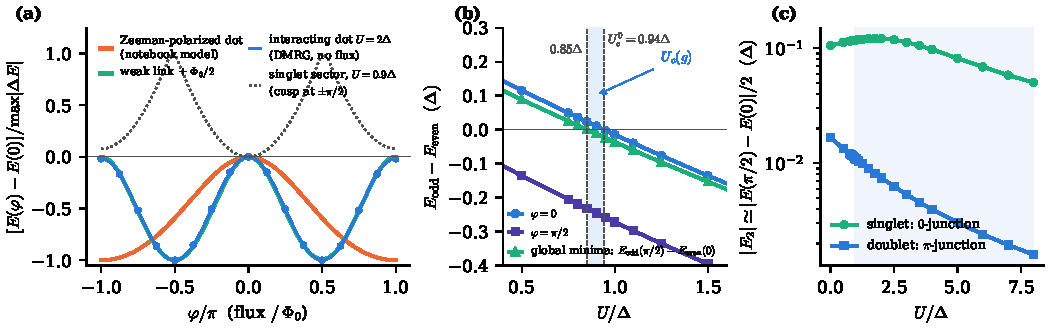
\includegraphics[width=\textwidth]{../figs/fig_junctions.pdf}
  \caption{\label{fig:junctions}%
  (a) Normalized $E(\varphi)$ of the loop for a Zeeman-polarized dot in a short ring (dominated by the
  $h/e$ harmonic), a weak link biased by $\Phi_0/2$ ($L=14$) and the interacting dot at $U=2\Delta$ without
  bias ($L=10$; symbols: DMRG; line: cosine fit); dotted: the singlet surface at $U=0.9\Delta$ with its cusp.
  (b) $E_{\rm odd}-E_{\rm even}$ at $\varphi=0$, at $\varphi=\pi/2$ and between the global minima
  (DMRG, $L=10$, $t_J=0.5\Delta$); shaded: the $\pi'$ window in which the boundary of the loop moves with $g$.
  (c) $|E_2|$ in the singlet and doublet sectors.}
\end{figure*}

\paragraph*{S3. DMRG protocol.}
The ring is stored in folded order next to the bosonic site, so that all ring bonds have range $\le2$
and the vertex $Dc^\dagger_{1\sigma}c_{0\sigma}$ is a three-site operator. Fermion parity and $S^z$ are
conserved. Benchmarks: at $g=0$ the energies of the non-interacting ring agree with exact BdG to
$10^{-14}$ at $\chi=1024$; for a four-site ring with a photon, DMRG reproduces exact diagonalization and the
sum rule $\langle I\rangle=(e/\hbar)(\hbar\omega/2g)\langle X\rangle$ to $10^{-7}$. On the phase diagram
$\chi=300$ (truncation error $<2\times10^{-8}$; $\chi=400$ changes the energies by $<4\times10^{-8}\Delta$ and
the current by $<0.3\%$ away from the crossover points) and $N_{\rm ph}=50$--$62$ (last Fock weight
$<10^{-7}$; $N_{\rm ph}=80$ changes the energy by $<10^{-9}\Delta$). The relevant criterion is not the energy:
the two current states are split only by $\delta$ and by the seed, $2I^\star\varphi_{\rm cl}\sim10^{-5}\Delta$,
and the local updates of DMRG drift towards the polarized state over tens of sweeps and can stop in an
under-polarized state whose energy is within $10^{-6}\Delta$ of the ground state. Every seeded point is
therefore started from two independent states, a warm start from the neighbouring point on the vacuum side
and a product state with the mode in a coherent state at the classical flux, converged first with seeds
$10^{-2}$ and $3\times10^{-3}$ and then relaxed at $10^{-3}$; the lower energy is kept when the two differ by
more than $3\times10^{-7}\Delta$, otherwise the pair is reported as a bracket ($47$ of $427$ points, all inside
the crossover windows); a state is accepted only if it satisfies the sum rule to $10^{-3}I_c$ (median
$10^{-4}I_c$); and the current above threshold must be independent of the seed (seed $10^{-4}$: unchanged to
$0.4\%$ above threshold, reduced by the factor $0.09$ below) [Fig.~\ref{fig:phaseconv}]. An earlier version
of these scans evaluated the observables after a warm start with the displacement operator of the previous
$g$; the sum rule exposed this error. For the seed-free runs (cat state, flux-driven switch) the symmetric
state is the ground state in each sector and no such care is needed; on the grid of Fig.~2 ($\hbar\omega=0.01$--$3\Delta$, $\chi=200$,
$N_{\rm ph}=16$--$48$) the truncation error is $<4\times10^{-7}$ and the last Fock weight $<4\times10^{-8}$, and the
boundary $U_c$ is obtained by linear interpolation of $E_{\rm odd}-E_{\rm even}$ between $U$ nodes $0.1$--$0.2\Delta$ apart
(adding nodes $0.05$--$0.1\Delta$ apart moves $U_c$ by $<10^{-3}\Delta$; $\chi=300$ changes the energies by $<5\times10^{-6}\Delta$ and the
difference by $<4\times10^{-6}\Delta$, $N_{\rm ph}=40$--$80$ by $<10^{-7}\Delta$); the photon--electron entanglement
entropy is computed from the photon reduced density matrix. The circuit model is diagonalized in a Fock
space of $200$ states (DVR in the eigenbasis of $X$); for the tunnel splitting below $10^{-6}\hbar\omega$ the
two flux-parity blocks are diagonalized separately, which gives $\delta$ as a difference of two
independently converged energies ($6.46\times10^{-9}\hbar\omega$ against $6.51\times10^{-9}$ from the full matrix
at $\beta=3$, $E_J/\hbar\omega=10$; at $E_J/\hbar\omega=40$ both are at the double-precision floor
$\sim10^{-9}\hbar\omega$ for $\beta\ge1.25$).

\begin{figure*}
  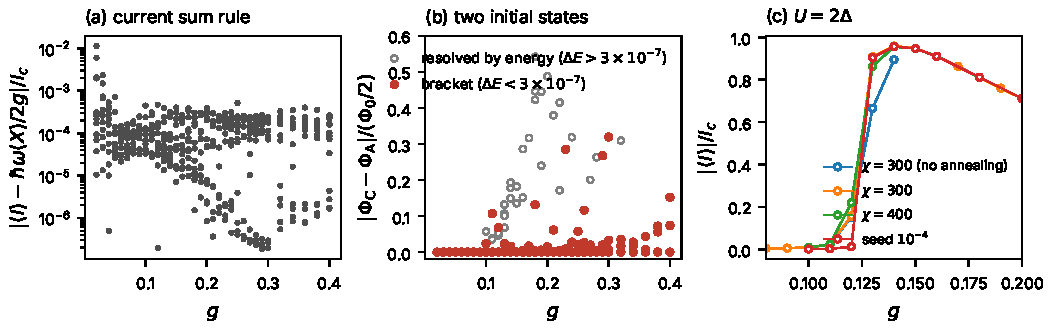
\includegraphics[width=\textwidth]{../figs/fig_phase_convergence.pdf}
  \caption{\label{fig:phaseconv}%
  Convergence of the full DMRG on the phase diagram. (a) Violation of the sum rule over the grid.
  (b) Difference between the fluxes of the two initial states (vacuum side A, polarized side C) in units of
  $\Phi_0/2$: open symbols resolved by the energy, filled reported as brackets. (c) $U=2\Delta$ near threshold:
  $\chi=300$ without and with the annealed start, $\chi=400$, and seed $10^{-4}$.}
\end{figure*}


\begin{figure*}
  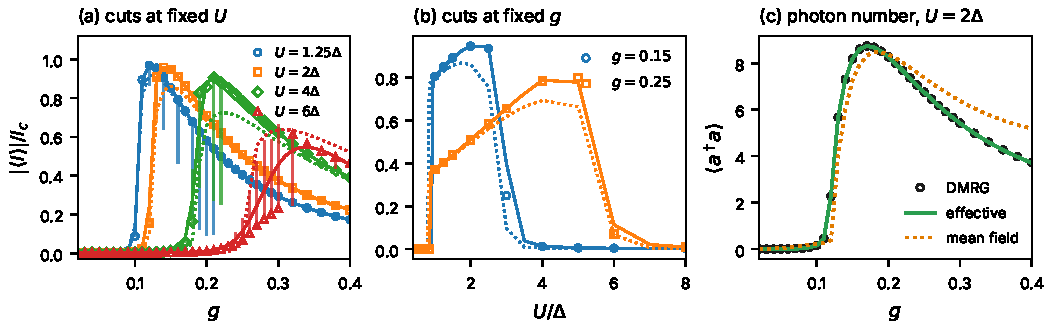
\includegraphics[width=\textwidth]{../figs/fig_phase_slices.pdf}
  \caption{\label{fig:phaseslices}%
  Cuts through Fig.~2 of the main text. (a) Current versus $g$ at $U/\Delta=1.25,2,4,6$ and (b) versus
  $U$ at $g=0.15,0.25$: full DMRG (symbols; bars: bracket between the two initial states), circuit model
  (solid), mean field (dotted). (c) Photon number at $U=2\Delta$.}
\end{figure*}

\paragraph*{S4. Half-flux-biased weak link.}
For an ordinary weak link ($L=14$, $t_J=0.5$, $E_2=-0.056\Delta$, $E_1=-5.4\times10^{-4}\Delta$, Andreev gap
$0.77\Delta$) biased by $\Phi_0/2$, Fig.~\ref{fig:halfflux} shows the full DMRG at $E_J/\hbar\omega=10$ versus
$\beta$. The current rises at $\beta\simeq1.1$, saturates at $0.96I_c$ for $\beta\approx1.7$ and then
decreases as the flux approaches $\Phi_0/2$. DMRG and the circuit model agree to $2\times10^{-3}\hbar\omega$
in energy, $2\%$ of $I_c$ in current and $1.3\%$ in $E_1-E_0$. The product state is $0.2$--$0.4\hbar\omega$
too high in energy and overestimates the current threefold near threshold ($0.71I_c$ against $0.22I_c$ at
$\beta=1.13$). The direction of the current is selected by the residual $h/e$ harmonic, which tilts the double
well by $2|E_1|\sin\varphi^\star\approx0.2\hbar\omega$ and sets $E_1-E_0$ for $\beta>1.2$; without it
$\delta/\hbar\omega$ would fall below $10^{-6}$ at $\beta=2$. The flux distribution evolves from a Gaussian
at zero to a single displaced peak.

\begin{figure*}
  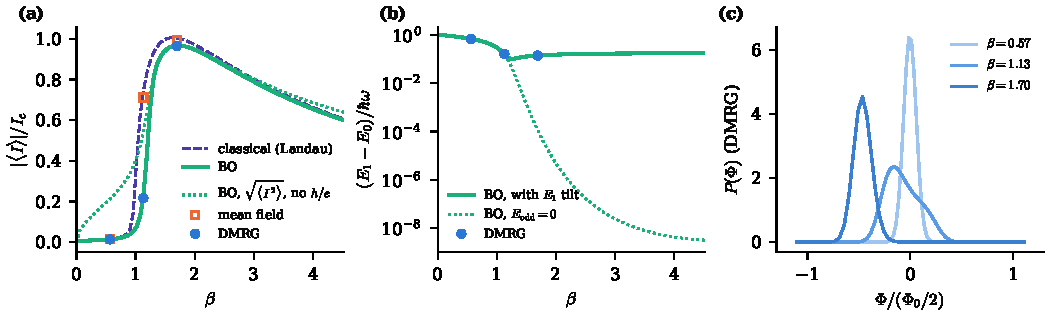
\includegraphics[width=\textwidth]{../figs/fig_weaklink_halfflux.pdf}
  \caption{\label{fig:halfflux}%
  Weak-link loop ($L=14$) biased by $\Phi_0/2$, $E_J/\hbar\omega=10$. (a) Persistent current versus $\beta$:
  DMRG (circles), MF (squares), circuit model with (solid) and without (dotted) the odd harmonics, classical
  Landau theory (dashed). (b) Splitting of the two lowest levels. (c) Flux distribution of the DMRG ground state.}
\end{figure*}

\paragraph*{S5. Product state at $E_J\simeq\hbar\omega$.}
The product-state mean field is the method of Refs.~\cite{Varrica2026,Andolina2020} and of our own earlier
treatment of this circuit: Hartree--Fock BdG electrons with the junction bond renormalized by
$\alpha=\langle D\rangle$, times the ground state of $\hbar\omega a^\dagger a-(\eta D+{\rm h.c.})$ with
$\eta=t_Je^{i\varphi}\langle c^\dagger_1c_0\rangle$, iterated to self-consistency. For a Zeeman-polarized dot
in a short BCS ring ($t=2$, $\Delta=0.6$, $L=11$, $\epsilon_{d\uparrow}=-0.3$, $\epsilon_{d\downarrow}=3.7$,
$t_J=0.5$, $\hbar\omega=0.02$; energies in units of $t$) it predicts a current-carrying phase for
$g\gtrsim0.75$ with $|\langle I\rangle|\approx0.02$ and $\langle a^\dagger a\rangle\simeq1$--$1.4$. DMRG shows
that this phase is an artefact [Fig.~\ref{fig:notebook}]: the exact energy lies below the MF energy by up to
$1.8\hbar\omega$, the gap to the first excited state stays at $0.33\hbar\omega$, the photon number saturates at
$0.36$ and the response to the seed is linear, $\langle I\rangle\approx7\times10^{-5}$. Two effects are
responsible. (i) The product state is not gauge covariant: with the full Peierls phase on one bond it
renormalizes that bond by $|\langle D\rangle|<1$ and loses phase-\emph{independent} kinetic energy, which the
exact state recovers by following the flux. (ii) $E_J\simeq\hbar\omega$: the Landau energy develops a double
well for $g>0.58$, but its depth is below the zero-point energy and $P(X)$ stays unimodal. In this ring
$L\lesssim\xi$ and $E(\varphi)$ is dominated by the $h/e$ harmonic ($E_1=2.1\times10^{-2}\gg E_2=2\times10^{-3}$),
which is why all other results use $L\gg\xi$. At $\hbar\omega=0.002$ the same model does order, at
$g_c\simeq0.21$, while mean field gives $0.30$.

\begin{figure}
  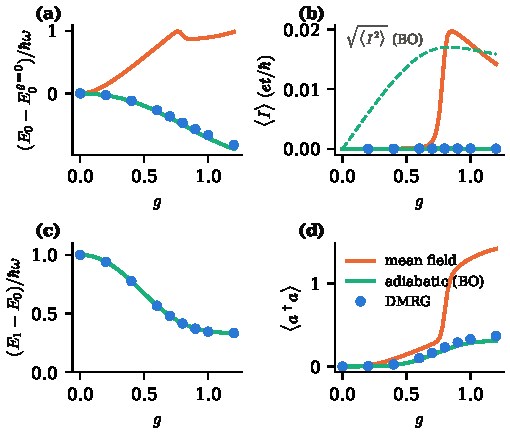
\includegraphics[width=\columnwidth]{../figs/fig_notebook_model.pdf}
  \caption{\label{fig:notebook}%
  Short ring with a Zeeman-polarized dot ($\hbar\omega=0.02$, seed $10^{-3}$): mean field (orange), circuit
  model (green) and DMRG (symbols). (a) Energy, (b) current (dashed: rms current of the circuit-model ground
  state), (c) gap to the first excited state, (d) photon number.}
\end{figure}

\paragraph*{S6. Physical units.}
With $E_J/h=0.5\,{\rm GHz}\times I_c[{\rm nA}]$ and $\beta=2\pi(Z/R_Q)(E_J/\hbar\omega)$:

\begin{center}\scriptsize
\begin{tabular}{lccccc}
\hline
junction, material & $E_J/h$ & $I_c$ & $E_J/10h$ & $E_J/10k_B$ & $L_{\beta=1}$ \\
\hline
$2\Delta$, $\Delta/2$, Al & 0.32 GHz & 0.65 nA & 32 MHz & 1.5 mK & 510 nH \\
$2\Delta$, $\Delta/2$, NbTiN & 2.1 GHz & 4.3 nA & 210 MHz & 10 mK & 76 nH \\
$6\Delta$, $2\Delta$, Al & 1.5 GHz & 3.0 nA & 150 MHz & 7 mK & 110 nH \\
$6\Delta$, $2\Delta$, NbTiN & 9.9 GHz & 20 nA & 0.99 GHz & 47 mK & 17 nH \\
$6\Delta$, $2\Delta$, Nb & 11.5 GHz & 23 nA & 1.15 GHz & 55 mK & 14 nH \\
\hline
\end{tabular}
\end{center}
(first column: $U$, $\Gamma$, superconductor; $L_{\beta=1}=\Phi_0/2\pi I_c$).
The flux-driven switch needs none of this: $\hbar\omega=0.1\Delta$ is $4.4$\,GHz in Al and $g=0.5$ is
$Z=2.0\,{\rm k}\Omega$.
